\documentclass{beamer}
\usepackage[utf8]{inputenc}

\usetheme{Madrid}
\usecolortheme{default}
\usepackage{amsmath,amssymb,amsfonts,amsthm}
\usepackage{txfonts}
\usepackage{tkz-euclide}
\usepackage{listings}
\usepackage{adjustbox}
\usepackage{array}
\usepackage{tabularx}
\usepackage{gvv}
\usepackage{lmodern}
\usepackage{circuitikz}
\usepackage{tikz}
\usepackage{graphicx}
\usepackage{enumitem}

\setbeamertemplate{page number in head/foot}[totalframenumber]

\usepackage{tcolorbox}
\tcbuselibrary{minted,breakable,xparse,skins}



\definecolor{bg}{gray}{0.95}
\DeclareTCBListing{mintedbox}{O{}m!O{}}{%
  breakable=true,
  listing engine=minted,
  listing only,
  minted language=#2,
  minted style=default,
  minted options={%
    linenos,
    gobble=0,
    breaklines=true,
    breakafter=,,
    fontsize=\small,
    numbersep=8pt,
    #1},
  boxsep=0pt,
  left skip=0pt,
  right skip=0pt,
  left=25pt,
  right=0pt,
  top=3pt,
  bottom=3pt,
  arc=5pt,
  leftrule=0pt,
  rightrule=0pt,
  bottomrule=2pt,
  toprule=2pt,
  colback=bg,
  colframe=orange!70,
  enhanced,
  overlay={%
    \begin{tcbclipinterior}
    \fill[orange!20!white] (frame.south west) rectangle ([xshift=20pt]frame.north west);
    \end{tcbclipinterior}},
  #3,
}
\lstset{
    language=C,
    basicstyle=\ttfamily\small,
    keywordstyle=\color{blue},
    stringstyle=\color{orange},
    commentstyle=\color{green!60!black},
    numbers=left,
    numberstyle=\tiny\color{gray},
    breaklines=true,
    showstringspaces=false,
}
%------------------------------------------------------------
%This block of code defines the information to appear in the
%Title page
\title %optional
{4.3.41}
\date{October 2, 2025}

\author 
{Shreyas Goud Burra - EE25BTECH11051}
\begin{document}

\frame{\titlepage}

\begin{frame}{Question}
The cartesian equation of a line is $\frac{x-5}{3}=\frac{y+4}{7}=\frac{z-6}{2}$. Write its vector form.
\end{frame}
\begin{frame}{Given Information}
Given cartesian equation of line is

\begin{align}
    \frac{x-5}{3}=\frac{y+4}{7}=\frac{z-6}{2}=\lambda
    \label{0.1}
\end{align}

We know the vector form of a line is given by,
\begin{align}
    \textbf{x} = \textbf{h}+k\textbf{m}
    \label{0.2}
\end{align}
\end{frame}
\begin{frame}{Solution}
Where \textbf{x} is a point on the given line, \textbf{h} is a known point on that line, \textbf{m} is the slope of the line and k is an arbitrary real constant.\\

From \ref{0.1}, we can determine a point on the line taking $\lambda =0$
\begin{align}
    \frac{x-5}{3}=\frac{y+4}{7}=\frac{z-6}{2}=0 \implies x=5, y=-4, z=6
    \label{0.3}
\end{align}

\begin{align}
    \implies \textbf{h} = \myvec{5\\-4\\6}
    \label{0.4}
\end{align}
\end{frame}

\begin{frame}{Final Answer}
We can get the ratio of direction cosines from \ref{0.1}
\begin{align}
    \text{ratio}=3:7:2 \implies \textbf{m} = \myvec{3\\7\\2}
    \label{0.5}
\end{align}

Substituting \ref{0.4} and \ref{0.5} in \ref{0.2}, we get

\begin{align}
    \textbf{x} = \myvec{3\\-4\\6} + k\myvec{3\\7\\2}
    \label{0.6}
\end{align}
\end{frame}

\begin{frame}[fragile]
\frametitle{Python code}
\begin{lstlisting}
import numpy as np
import matplotlib.pyplot as plt


t = np.linspace(-10, 10, 100)

m = np.array([3, 7, 2], dtype=np.float64)
x = 5 + t * m[0]
y = -4 + t * m[1]
z = 6 + t * m[2]


fig = plt.figure()
ax = plt.subplot(111, projection='3d')  

\end{lstlisting}
\end{frame}

\begin{frame}[fragile]
\frametitle{Python code}
\begin{lstlisting}


ax.plot(x, y, z, label='3D Line', color='blue')
ax.scatter(5, -4, 6, color='red', label='Point (5, -4, 6)')


ax.set_xlabel('X')
ax.set_ylabel('Y')
ax.set_zlabel('Z')
ax.legend()
ax.set_title('3D Line from Vector Equation')

\end{lstlisting}
\end{frame}

\begin{frame}[fragile]
\frametitle{Python code}
\begin{lstlisting}


plt.savefig('/home/shreyas/GVV_Assignments/matgeo/4.3.41/figs/fig1.png')
plt.show()

\end{lstlisting}
\end{frame}

\begin{frame}{3D Plot}
\begin{figure}[H]
    \centering
    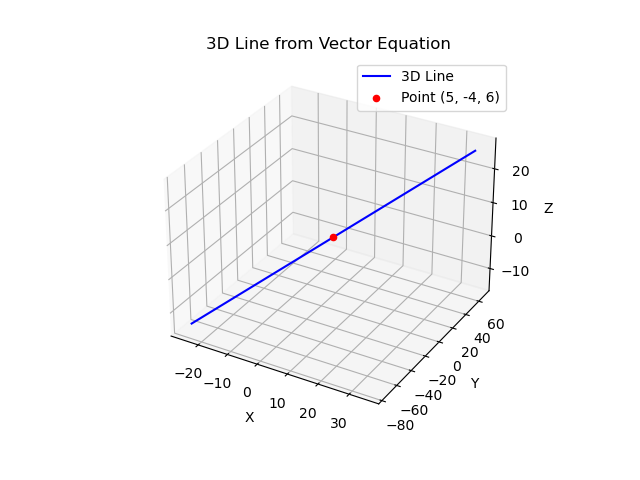
\includegraphics[width=0.8\columnwidth]{figs/fig1.png}
    \caption{3D Plot}
    \label{3D Plot}
\end{figure}
\end{frame}



\end{document}
